\section{method}
\subsection{Research Methods}
I will use a variety of of research methods during the internship.

For the choice of language, I will use a comparitive investigation.
For the other subquestions, I will use a combination of design and experimentation, as I use LEAN prototyping.

\subsection{Information collection}
I will mainly use the internet to find official documentation and to download international standards.
I will also use Google Scholar to find published papers.

\subsection{Validation of findings}
The correctness requirement will be validated by running test programs and comparing the output of the interpreter with the output of the compiler.
The generated code will also be inspected with a debugger to find code generation errors.
Performance requirements will be validated by

\subsection{Validity and reliability of sources}
I will use official documentation and international standards from ECMA International and ISO wherever possible.
The theory is also put in practice, providing evidence that the sources were sound.

\subsection{Project methods}
We will make use of LEAN Rapid Prototyping\cite{lean}.

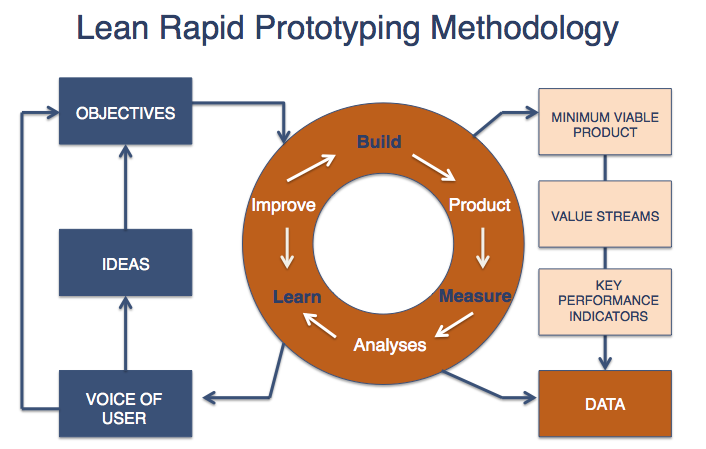
\includegraphics[width=\textwidth]{lean}

This method is great for small teams, as it reduces overhead.
This is crucial because we need to spend our time efficiently if we want to deliver a finished product.
It also allows us to gather knowledge by iterating over our designs.

\subsection{Risk assesment}
\begin{center}
   \begin{tabular}
      {| p{0.2\textwidth} | p{0.28\textwidth} | l | p{0.3\textwidth} |}
      \hline
      \textbf{Risk} & \textbf{Effect} & \textbf{Possibility} & \textbf{Counter measure} \\
      \hline
      No test programs will be available.  & 
	  No emperic mesurements can be done. & 
	  50\% & 
	  I will have to write test programs in the intermediate language \\
	  \hline
      The Type-Checker is not finished in time. &
	  No emperic mesurements on complex programs can't be done. & 
	  50\% & 
	  The complex programs will have to be manually converted to simple programs by me or members of the research-group. \\
      \hline
      The optimisations will not be enough to be faster than python. & 
	  The compiler will not be compettitive with other compilers & 
	  10\% & 
	  Investigate why and report. \\
	  \hline
      Parts are left unfinished due to time constraints. & 
	  Not all requirements will be met & 
	  20\% & 
	  Propper planning an prioritizing low hanging fruit can minimize this. \\
	  \hline
   \end{tabular}
\end{center}

\subsection{Quality expectations}
The quality expectations are encoded in the requirements.

